%%%%%%%%%%%%%%%%%%%%%%%%%%%%%%%%%%%%%%
\section{Experiments} \label{experiments}
%%%%%%%%%%%%%%%%%%%%%%%%%%%%%%%%%%%%%%
\begin{figure}[h]
    \centering
    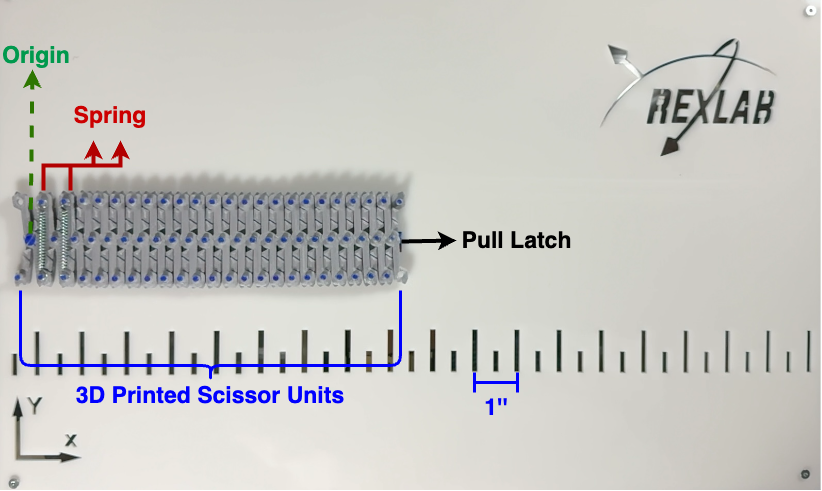
\includegraphics[width=\linewidth]{DOJO-CCK/Figures/scissor_hardware_setup.drawio.png}
    \caption{Hardware experimental setup with a 23-link scissor mechanism with joint clearance and friction. The mechanism has $n$ hook-law extension springs placed at the first $n$ cells of the scissor mechanism. A pull latch sets the mechanism under repeatable conditions, and an overhead high-speed camera captures the motion at 240 fps. The center and end locations of the scissor units are colored in blue to be detected using offline vision segmentation.}
    \label{fig:enter-label}
\end{figure}

\subsection{Simulation-to-Simulation Evaluation}

The digital twin framework was first evaluated using synthetic data in a simulation-to-simulation validation. The experiment comprised a 10-unit scissor mechanism with 0.001m joint tolerance and 0.01 N/m joint friction. This synthetic data served as ground truth for evaluating our estimation methods from visual data error estimation and system parameter identification. This experiment aimed to validate the accuracy of our estimation techniques in a controlled, noise-free environment before applying them to real hardware.

\subsubsection{Hardware Experiment}

A 3D-printed 23-unit scissor mechanism was analyzed to evaluate the efficacy on hardware data. The mechanical system was manufactured using PLA material on a Bambu FDM 3D printer. Springs were added at predefined locations to apply a known opening force, simulating real-world loading conditions. A laser-cut bed with measurement markers created a repeatable experiment environment. The motion of the scissor mechanism was captured using a slow-motion camera at 240 fps. The test bed was equipped with visual markings to convert pixel measurements into meters, facilitating data transfer from the hardware experiment to the simulation. 

% \subsection{Manufacturing and Physical Properties}

% The mechanical system was manufactured using PLA material on a Bambu FDM 3D printer. While the CAD model accurately captures geometrical and inertial properties, it fails to account for joint clearance and joint friction—parameters that can vary during manufacturing. These physical properties were measured and estimated after manufacturing to improve simulation accuracy.
% \subsection{Hardware Experiments with 3D Printed Mechanisms}

% Next, we conducted hardware experiments using 3D-printed versions of the scissor mechanism and the Bennett linkage. Each mechanism was evaluated using distinct experimental setups tailored to capture relevant kinematic and dynamic data.

% \subsubsection{Bennett Linkage Experiment}

% We also printed a 3D Bennett linkage fitted with motion capture markers placed on the coupler bar to track its motion. The linkage was actuated using a stepper motor controlled by an Arduino, operating at a fixed rotational speed of 5 revolutions per minute (RPM). The linkage movement was tracked using an Opti-Track motion capture system, providing high-fidelity position and orientation data for each moving part of the mechanism. This setup enabled the analysis of both kinematic parameters, such as joint clearance, and dynamic parameters, such as joint friction, based on the mechanism's real-world behavior.

% \subsubsection{Digital Twin Identification and Validation}

% The data was integrated into our digital twin framework after estimating the joint clearance and friction from the hardware experiments. The digital twins were validated by comparing the simulation outputs with the hardware measurements under known loading conditions. This comparison allowed us to assess how accurately the digital twin could replicate the physical system's performance.

\subsubsection{Jamming Experiments and Joint Reaction Force Analysis}
Finally, the observed jamming behavior on the hardware was analyzed using the digital twin. The analysis explores the system conditioning over time to the point of jamming and the joint reaction forces. The following section provides a discussion about the results. 

% were analyzed using the digital twins from the prior experiments. These conditions involved applying various forces and torques to simulate real-world scenarios where jamming might occur. We used the slow-motion camera and motion capture system to monitor and record any occurrences of jamming. In the digital twin, we tracked the appearance of additional singular values in the SVD-based model reduction, signaling a loss of degrees of freedom and the onset of jamming. By comparing the digital twin's predictions with real-world outcomes, we validated its ability to detect and analyze jamming behavior under different circumstances.
